% DO NOT COMPILE THIS FILE DIRECTLY!
% This is included by the other .tex files.



\begin{frame}[t,plain]
\titlepage
\end{frame}

%\begin{frame}[t]{}
%\vspace*{\fill}
%		Le train \� destination 
%\vspace*{\fill}
%\end{frame}

\begin{frame}[t]{Premier arr\^et : JGroups}
	\begin{center}
		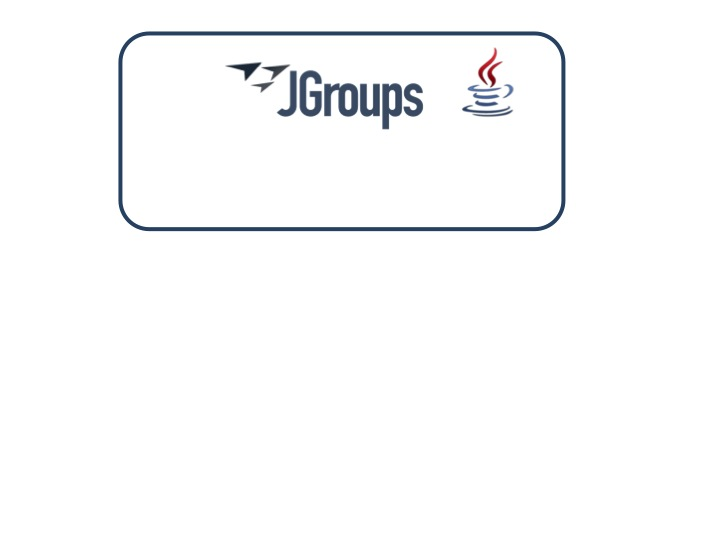
\includegraphics[scale=0.3]{img/schema/Diapositive01.jpg}
	\end{center}
\end{frame}

\begin{frame}[t]{Premier arr\^et : JGroups}
	\begin{center}
		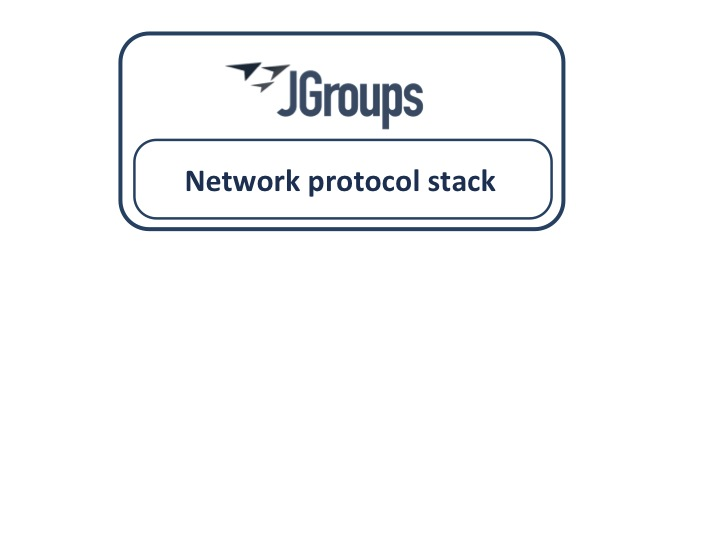
\includegraphics[scale=0.3]{img/schema/Diapositive02.jpg}
	\end{center}
\end{frame}

\begin{frame}[t]{Destination : int\'egrer le protocole des trains \`a JGroups}
	\begin{center}
		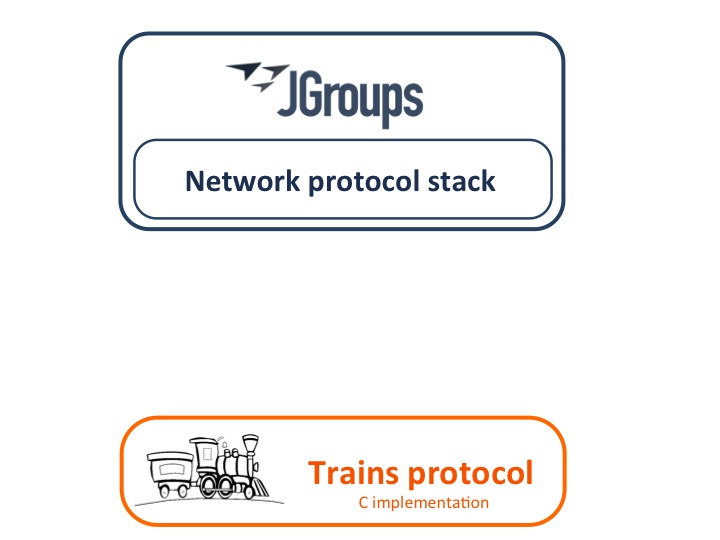
\includegraphics[scale=0.3]{img/schema/Diapositive03.jpg}
	\end{center}
\end{frame}

\begin{frame}[t]{Sommaire}
\begin{block}{Veuillez composter vos billets s'il vous pla\^it}
	\begin{enumerate}
	\item Introduction au protocole des trains
	\item Conception d'une API Java
	\item Int\'egration du protocole \`a JGroups
	\item Pour aller plus loin
	\item Conclusion
	\end{enumerate}
\end{block}	
\end{frame}

\begin{frame}[t]{Introduction au protocole des trains}
	\begin{block}{Tout le monde en voiture}
		~\\
	       \begin{itemize}
	       		\item Le protocole des trains est un protocole de \textbf{diffusion} (broadcast) :
			\begin{itemize}
				\item \textbf{uniforme}
				\item \textbf{totalement ordonn\'e}
			\end{itemize}
			\item Il permet d'obtenir un d\'ebit optimal.
		\end{itemize}
	\end{block}
\end{frame}

\begin{frame}[t]{Introduction au protocole des trains}
	\begin{block}{Tout le monde en voiture}
	      ~\\
	       \begin{itemize}
			\item Il est con\c{c}u pour :
				\begin{itemize}
					\item des petits clusters (16 machines maximum)
					\item des messages courts
				\end{itemize}
		\end{itemize}
	\end{block}
\end{frame}


\begin{frame}[t]{Le principe du protocole}
	\begin{block}{Le circuit}
		\begin{center}
			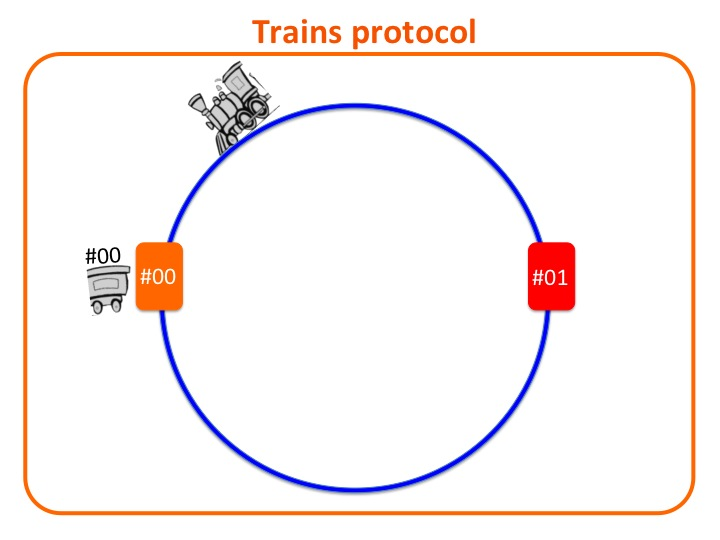
\includegraphics[scale=0.3]{img/schema/Diapositive11.jpg}
		\end{center}
	\end{block}
\end{frame}

\begin{frame}[t]{Le principe du protocole}
	\begin{block}{Envoi d'un message par \#00}
		\begin{center}
			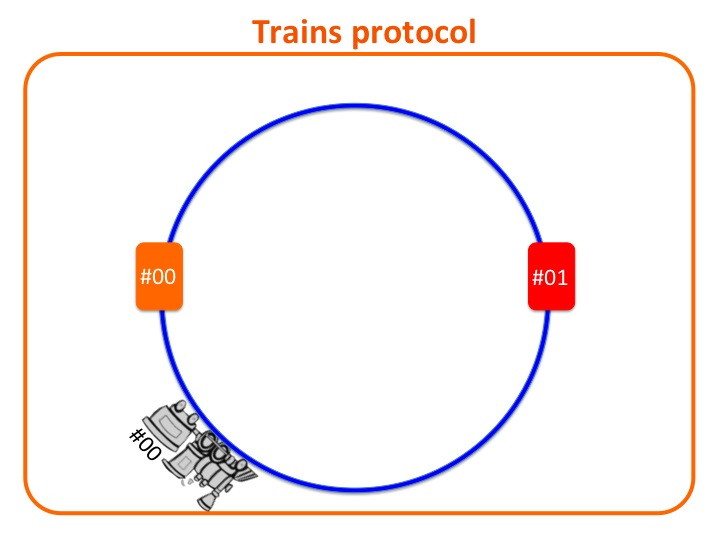
\includegraphics[scale=0.3]{img/schema/Diapositive12.jpg}
		\end{center}
	\end{block}
\end{frame}


\begin{frame}[t]{Le principe du protocole}
	\begin{block}{Diffusion du message - r\'eception par \#01}
		\begin{center}
			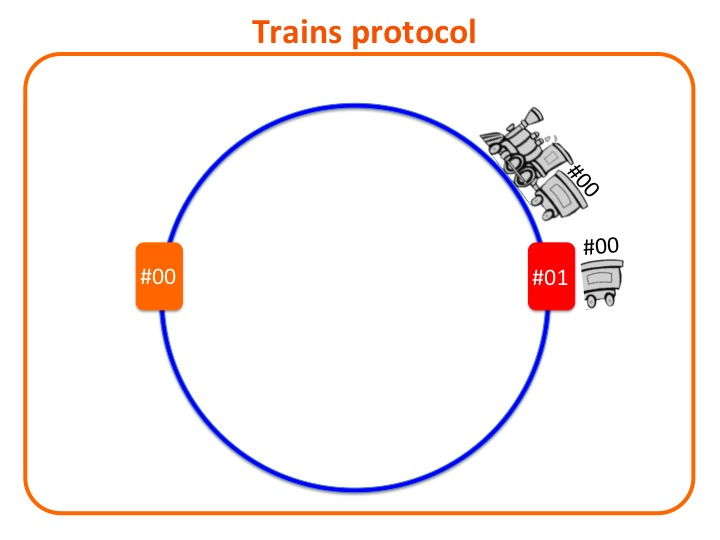
\includegraphics[scale=0.3]{img/schema/Diapositive13.jpg}
		\end{center}
	\end{block}
\end{frame}


\begin{frame}[t]{Le principe du protocole}
	\begin{block}{Suppression du wagon}
		\begin{center}
			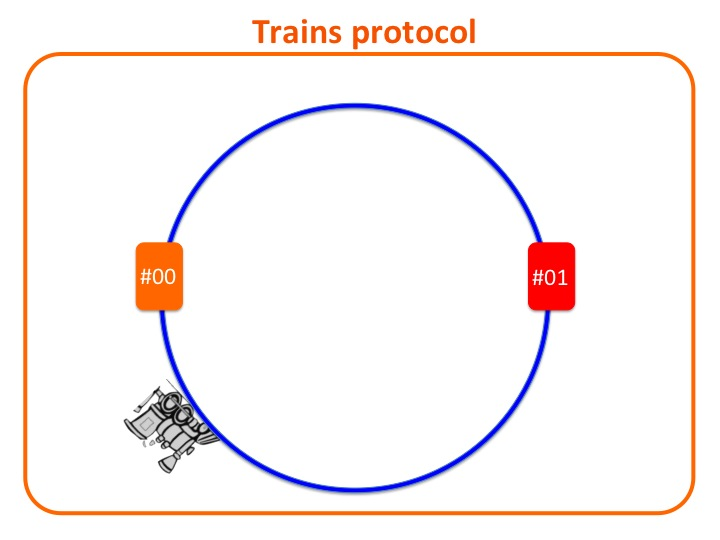
\includegraphics[scale=0.3]{img/schema/Diapositive14.jpg}
		\end{center}
	\end{block}
\end{frame}


\begin{frame}[t]{Le principe du protocole}
	\begin{block}{Arriv\'ee d'un nouveau processus}
		\begin{center}
			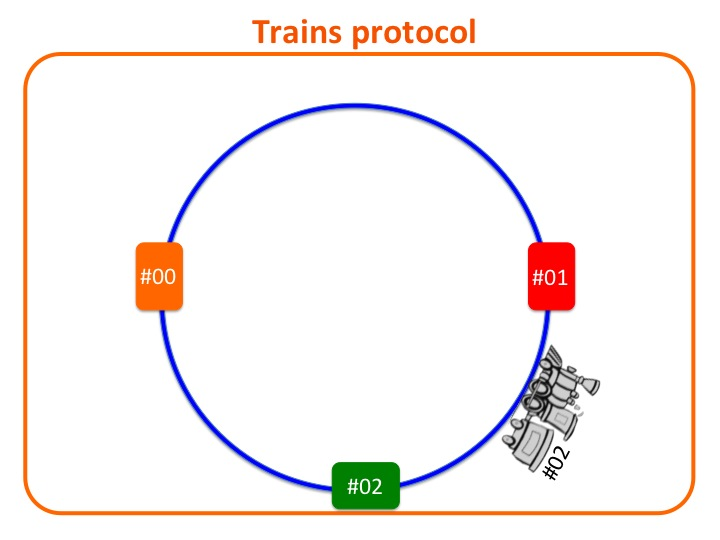
\includegraphics[scale=0.3]{img/schema/Diapositive15.jpg}
		\end{center}
	\end{block}
\end{frame}


\begin{frame}[t]{Impl\'ementation du protocole des trains en langage C}
	\begin{block}{Un fichier de configuration minimal}
		\begin{center}
		\begin{itemize}
				\item Fichier addr\_file : \\
				\textit{0:localhost:2000\\
				1:localhost:2001}
			\end{itemize}
		\end{center}
	\end{block}
\end{frame}

\begin{frame}[t]{Impl\'ementation du protocole des trains en langage C}
	\begin{block}{Un fichier de configuration minimal}
	\end{block}
	
	\begin{block}{Une interface simple}
		\begin{center}
			\begin{itemize}
				\item \textbf{Initialisation} : trInit()
				\item \textbf{Arr\^et} : trTerminate()
				\item \textbf{Cr\'eation d'un message} : newmsg()
				\item \textbf{Diffusion d'un message} : utoBroadcast()
				\item 3 structures : \textbf{message}, \textbf{messageHeader}, \textbf{circuitView}
			\end{itemize}
		\end{center}
	\end{block}
\end{frame}


\begin{frame}[t]{Pause au wagon-bar}
	\begin{block}{O\`u l'on doit faire du caf\'e}
		\begin{center}
			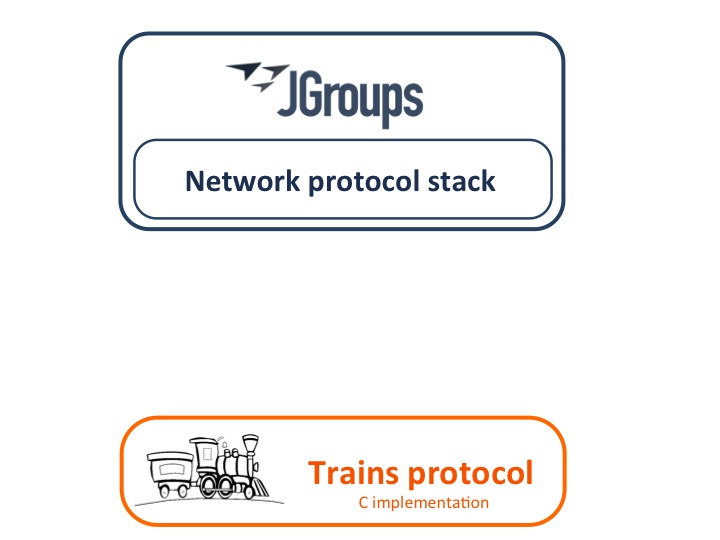
\includegraphics[scale=0.3]{img/schema/Diapositive03.jpg}
		\end{center}
	\end{block}
\end{frame}

\begin{frame}[t]{Pause au wagon-bar}
	\begin{block}{O\`u l'on doit faire du caf\'e}
		\begin{center}
			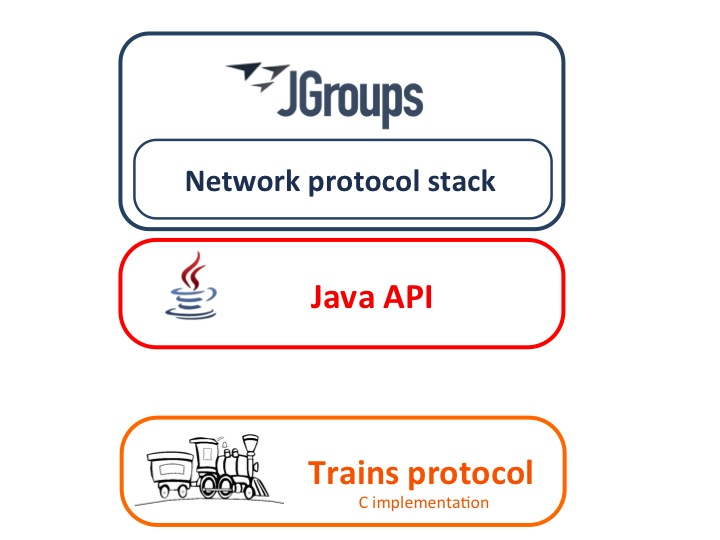
\includegraphics[scale=0.3]{img/schema/Diapositive04.jpg}
		\end{center}
	\end{block}
\end{frame}

\begin{frame}[t]{Pause au wagon-bar}
	\begin{block}{O\`u l'on doit faire du caf\'e}
		\begin{center}
			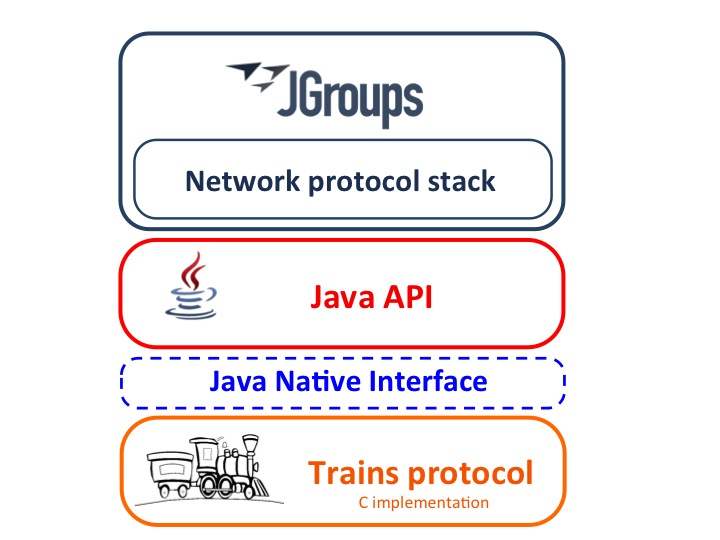
\includegraphics[scale=0.3]{img/schema/Diapositive05.jpg}
		\end{center}
	\end{block}
\end{frame}

\begin{frame}[t]{Java Native Interface}
		\begin{center}
			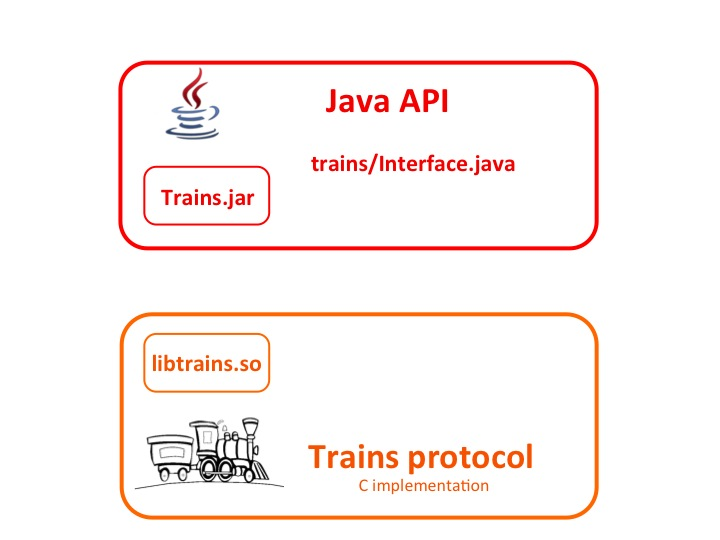
\includegraphics[scale=0.36]{img/schema/Diapositive06.jpg}
		\end{center}
\end{frame}

\begin{frame}[t]{Java Native Interface}
		\begin{center}
			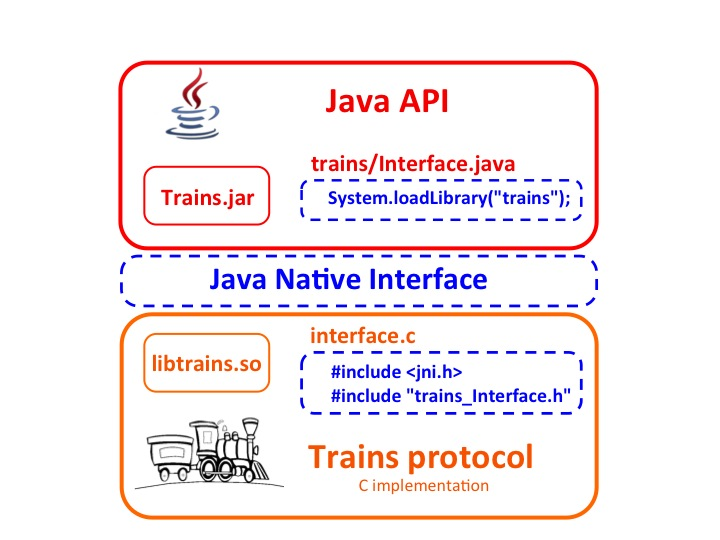
\includegraphics[scale=0.36]{img/schema/Diapositive07.jpg}
		\end{center}
\end{frame}

\begin{frame}[t]{Java Native Interface}
	\begin{block}{Avantages}
		\begin{itemize}
			\item Int\'eragir avec du code natif (C/C++)
				\begin{itemize}
					\item Acc\'eder \`a des fonctions syst\`emes
					\item Gestion du hardware
					\item Utilisation de librairies existantes
					\item Gain en performance (?)
				\end{itemize}
		\end{itemize}
	\end{block}
\end{frame}

\begin{frame}[t]{Java Native Interface}
	\begin{block}{Avantages}
	\end{block}
	\begin{block}{Inconv\'enients}
		\begin{itemize}
			\item Portabilit\'e d\'ependante du code natif
			\item Debug au run time difficile pour le code natif
			\item Gestion des vuln\'erabilit\'e du code natif
				\begin{itemize} 
					\item Gestion de la m\'emoire
				\end{itemize}
			\item Perte de performance
		\end{itemize}
	\end{block}
\end{frame}

\begin{frame}[t]{}
		\begin{center}
			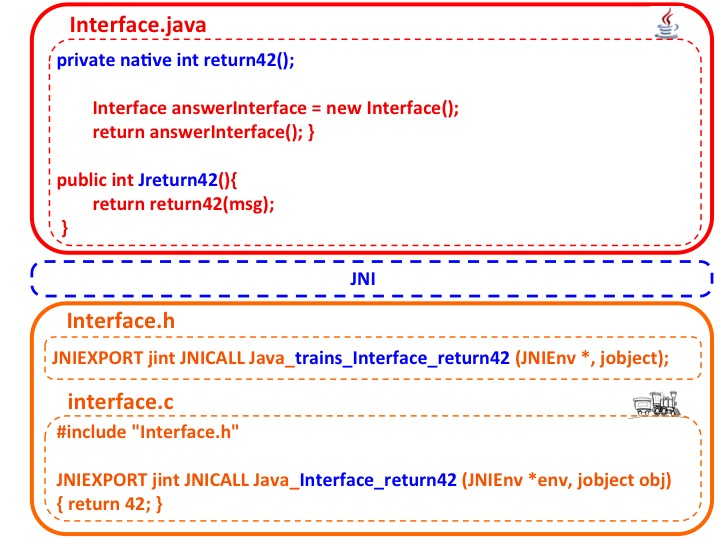
\includegraphics[scale=0.4]{img/schema/Diapositive09.jpg}
		\end{center}
\end{frame}

\begin{frame}[t]{API Java : trains}
		\begin{center}
			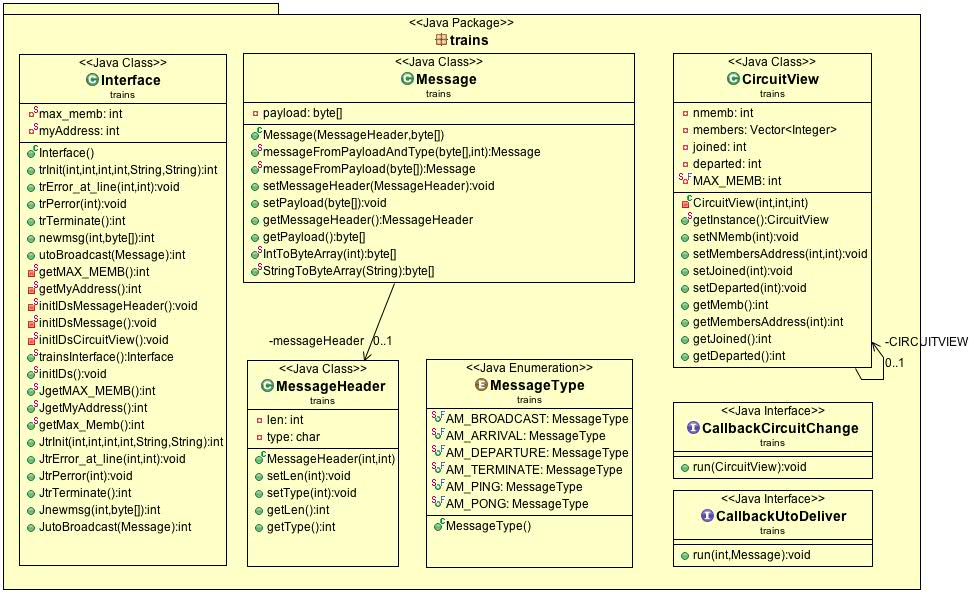
\includegraphics[scale=0.31]{img/trainsInterface.jpg}
		\end{center}
\end{frame}

\begin{frame}[t]{API Java : exemple}
		\begin{center}
			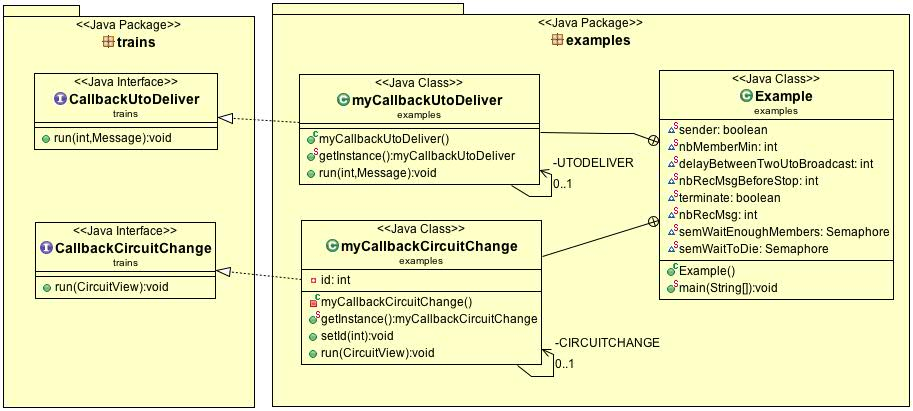
\includegraphics[scale=0.35]{img/example.jpg}
		\end{center}
\end{frame}

\begin{frame}[t]{Comparaison des performances}
		\begin{center}
			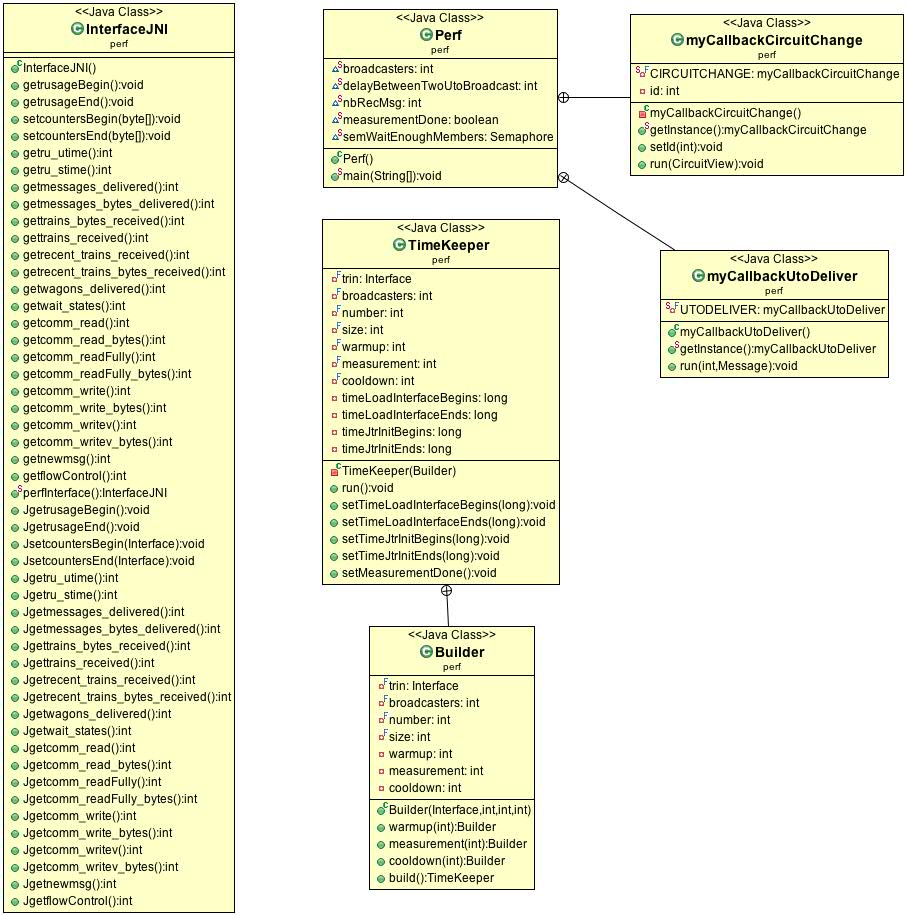
\includegraphics[scale=0.21]{img/perf.jpg}
		\end{center}
\end{frame}

\begin{frame}[t]{Comparaison des performances}
		\begin{center}
			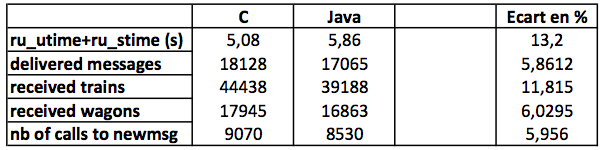
\includegraphics[scale=0.5]{img/perf.png}
			
			\begin{itemize}
				\item 1 train
				\item 2 processus en localhost, diffuseurs
				\item taille des messages: 10 octets
				\item dur�e de la mesure: 10 secondes (warmup: 1s, cooldown: 1s)
        \item 1 ms de d<8e>lai entre 2 envois de messages
			\end{itemize}
		\end{center}
\end{frame}

\begin{frame}[t]{Br\`eve introduction \`a JGroups}
    \begin{block}{JGroups}
        \begin{itemize}
            \item Intergiciel pour faire de la diffusion fiable
            \item Pile de protocoles flexible et configurable via un fichier
        \end{itemize}
    \end{block}
\end{frame}

\begin{frame}[t]{Br\`eve introduction \`a JGroups}
    \begin{block}{JGroups}
    \end{block}
    \begin{block}{Fonctionalit\'es}
        \begin{itemize}
            \item D\'etection et notification de l'arriv\'e et du d\'epart des membres
            \item D\'etection et enl\`evement des membres \'ecras\'es
            \item Envoi et r\'eception des message diffus\'e
            \item Envoi et r\'eception des message point-\`a-point
            \item Transfert d'\'etat
        \end{itemize}
    \end{block}
\end{frame}

\begin{frame}[t]{Br\`eve introduction \`a JGroups}
    \begin{block}{Architecture de la pile de protocoles}
        \begin{itemize}
            \item FLUSH / STATE TRANSFER
            \item Fragmentation (FRAG)
            \item Contr\^ole de flux (UFC, MFC)
            \item Contr\^ole d'appartenance dans group (GMS)
            \item Transfert fiable (STABLE, UNICAST2, etc)
            \item D\'etection des \'ech\`ecs (FD SOCK, VERIFY SUSPECT, etc)
            \item Merge des sous-groupes (MERGE)
            \item D\'ecouverte des membres (PING)
            \item Protocole de transfer (UDP, TCP)
        \end{itemize}
    \end{block}
\end{frame}

\begin{frame}[t]{Int\'egration \`a JGroups}
    \begin{block}{Objectif}
        \begin{itemize}
            \item Cr\'eation d'un protocole "trains" dans JGroups
            \item Permettre aux utilisateurs de switcher sur le protocole des trains sans toucher \`a leur code.
        \end{itemize}
    \end{block}
\end{frame}

\begin{frame}[t]{Int\'egration \`a JGroups}
    \begin{block}{Objectif}
    \end{block}

    \begin{block}{Fonctionalit\'es}
        \begin{itemize}
            \item D\'etection et notification de l'arriv\'e et du d\'epart des membres (pour les membres pr\'esents dans la liste)
            \item Envoi et r\'eception des messages diffus\'es
            \item Transfert d'\'etat
        \end{itemize}
    \end{block}
    
    \begin{block}{Simplifications}
        \begin{itemize}
            \item D\'etection et enl\`evement des membres \'ecras\'es
            \item Envoi et r\'eception des messages point-\`a-point
        \end{itemize}
    \end{block}
\end{frame}

\begin{frame}[t]{Int\'egration \`a JGroups}
    \begin{block}{Objectif}
    \end{block}

    \begin{block}{Fonctionalit\'es}
    \end{block}

    \begin{block}{Simplification}
    \end{block}

    \begin{block}{Architecture de la pile de protocoles}
        \begin{itemize}
            \item FLUSH / STATE TRANSFER
            \item Trains protocol
        \end{itemize}
    \end{block}
\end{frame}

\begin{frame}[t]{D\'emonstration}
		\begin{center}
		\end{center}
\end{frame}

\begin{frame}[t]{Bilan : terminus tout le monde descend}
	\begin{block}{Objectifs atteints}
		\begin{itemize}
			\item API Java avec JNI op\'erationnelle
			\item Int\'egration d'une brique protocolaire dans JGroups fonctionnelle
			\item Transfert d'\'etat en marche
		\end{itemize}
	\end{block}
\end{frame}

\begin{frame}[t]{Bilan : terminus tout le monde descend}
	\begin{block}{Objectifs atteints}
	\end{block}
	\begin{block}{Prochaines \'etapes}
		\begin{itemize}
			\item Compatibilit\'e du protocole avec Windows (et BSD ?)
			\item Calcul plus fin des performances
		\end{itemize}
	\end{block}
\end{frame}



